\setcounter{figure}{0}\setcounter{table}{0}
\renewcommand{\thefigure}{A\arabic{figure}}\renewcommand{\thetable}{A\arabic{table}}
\phantomsection
\section*{Additional Figures and Tables}
\addcontentsline{toc}{section}{Additional Figures and Tables}

\begin{table}[H]
\centering
\small
\begin{minipage}[t]{0.5\textwidth}
\centering\small\setlength{\tabcolsep}{4pt}
\begin{tabular}{lccc}
\toprule
Method & Clusters & Silhouette & ARI \\
\midrule
k-means & 2 & \textbf{0.278} & 0.299 \\
Hierarchical (Ward) & 2 & 0.205 & \textbf{0.867} \\
Gaussian mixture & 2 & 0.213 & 0.342 \\
DBSCAN & 1 + 63\% noise & -- & 0.68 \\
\bottomrule
\end{tabular}
\end{minipage}\hfill
\begin{minipage}[t]{0.48\textwidth}
\centering\small\setlength{\tabcolsep}{4pt}
\begin{tabular}{lcc}
\toprule
Features used & Count & ARI \\
\midrule
All & 30 & 0.867 \\
Without duplicated logs & 28 & 0.480 \\
Original only & 24 & 0.950 \\
Numeric only & 20 & 0.480 \\
Binary (0/1) only & 10 & 0.743 \\
One removed (30 runs) & 29 & 0.45--0.95 \\
\bottomrule
\end{tabular}
\end{minipage}
\caption{Clustering of the 320 training patients. Left: the four methods. Right: hierarchical clustering on other feature sets.}
\label{tab:clust}
\end{table}

\begin{figure}[H]
\centering
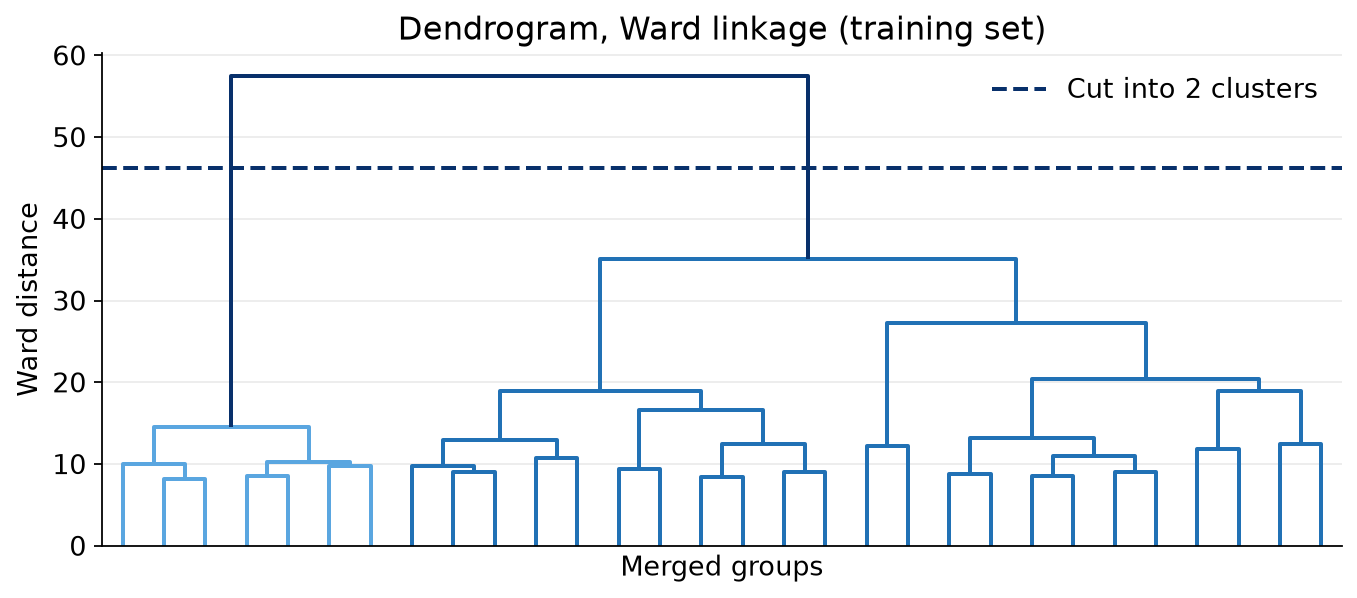
\includegraphics[width=0.78\textwidth]{figures/clustering_dendrogram.png}\\[8pt]
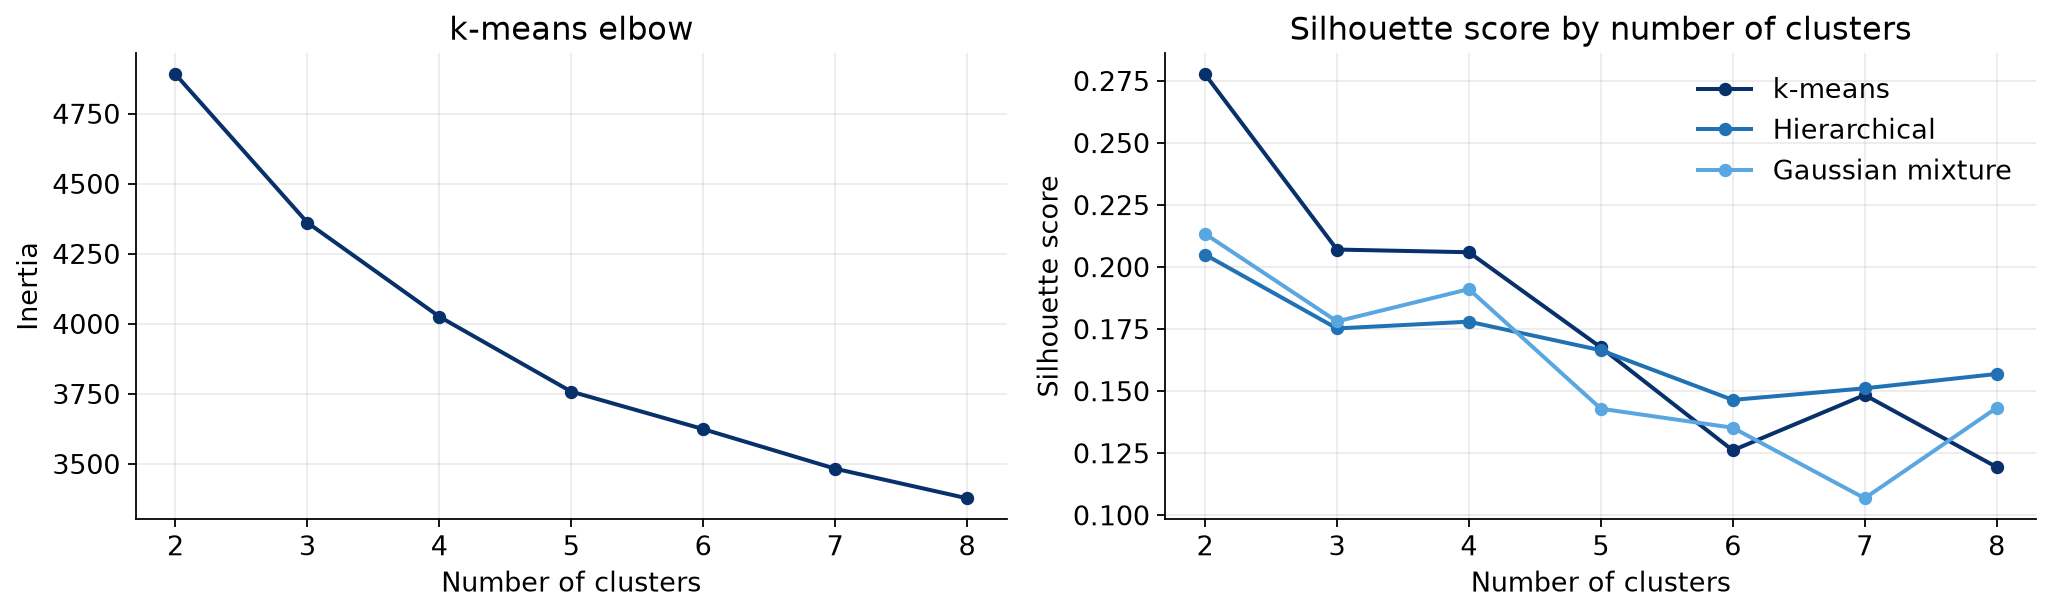
\includegraphics[width=\textwidth]{figures/clustering_k.png}
\caption{Choosing the number of clusters: Ward dendrogram (top), k-means inertia and silhouette score (bottom).}
\label{fig:clusterk}
\end{figure}

\begin{figure}[H]
\centering
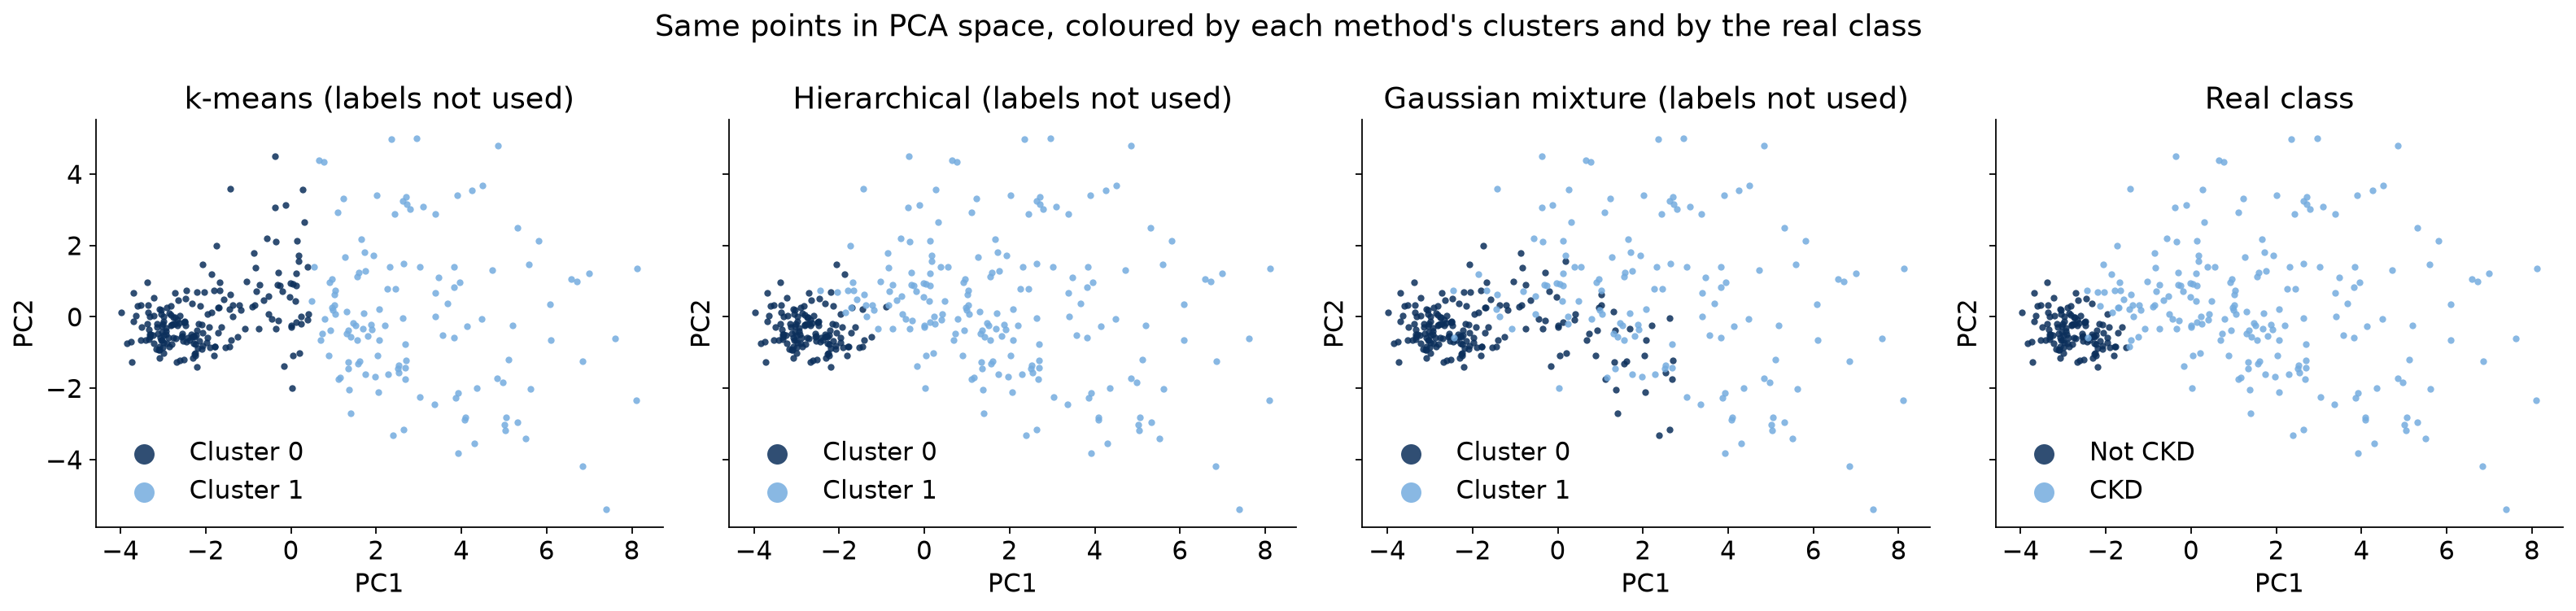
\includegraphics[width=\textwidth]{figures/clustering_pca.png}
\caption{Training patients in PCA space, coloured by each method's two clusters and by the real class.}
\label{fig:clusters}
\end{figure}

\clearpage

\begin{table}[H]
\centering
\footnotesize\setlength{\tabcolsep}{4pt}
\begin{tabular}{llcc@{\hskip 1.2em}llcc}
\toprule
Model & Version & CV & Test & Model & Version & CV & Test \\
\midrule
kNN & Baseline ($k=5$, 30 features) & 0.974 & 0.987 & Naive Bayes & Default, 30 features & 0.961 & 0.974 \\
 & Tuned, 30 features & 0.976 & 1.000 & & Tuned smoothing & 0.960 & 0.961 \\
 & \textbf{Tuned, 15 selected features} & \textbf{0.993} & 1.000 & & \textbf{3 selected features} & \textbf{0.966} & 0.933 \\
 & Selection + cluster label & 0.988 & 1.000 & & Mixed Gaussian + Bernoulli & 0.953 & 0.987 \\
Decision Tree & Fully grown & 0.978 & 0.973 & Random Forest & \textbf{300 trees, 15 features} & \textbf{0.993} & 0.987 \\
 & Grid-tuned & 0.973 & 0.946 & & & & \\
 & \textbf{Pruned} & \textbf{0.979} & 0.959 & & & & \\
\bottomrule
\end{tabular}
\caption{All versions of the classical models on DS1: macro F1 in repeated CV and on the test set (final in bold).}
\label{tab:versions}
\end{table}

\begin{figure}[H]
\centering
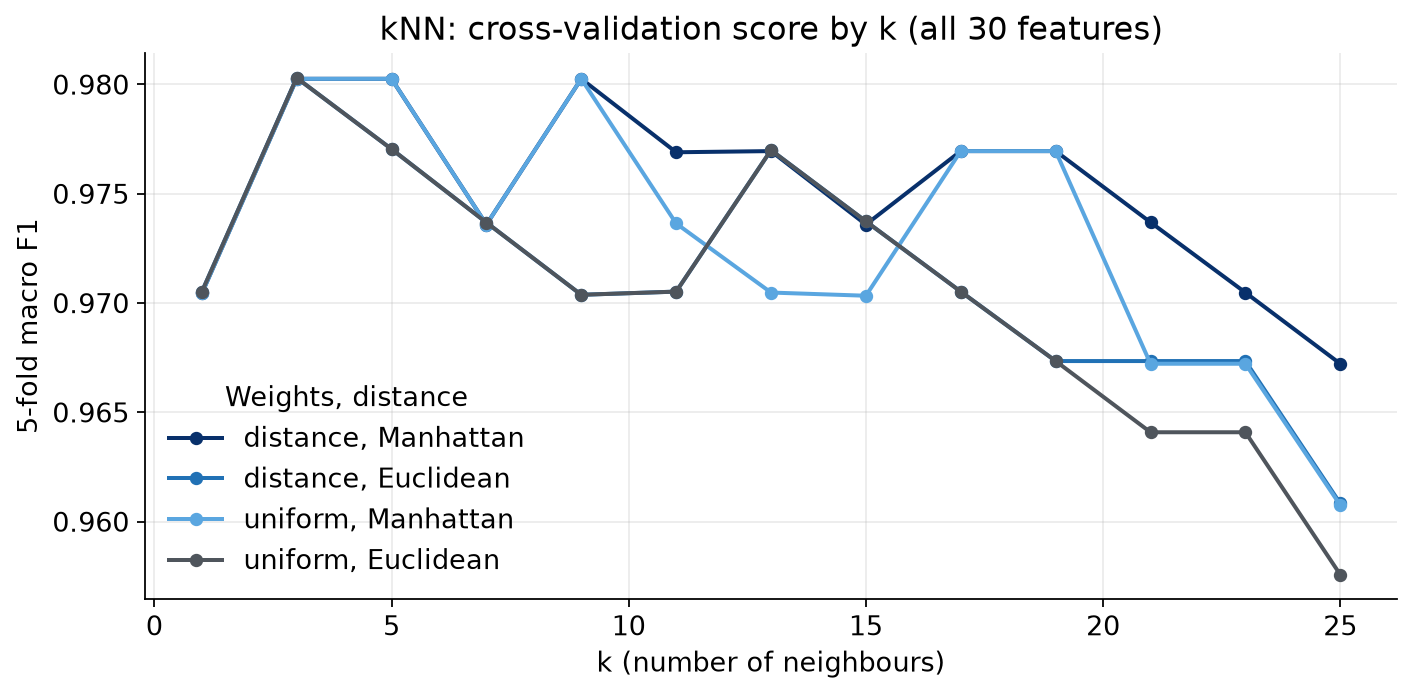
\includegraphics[width=0.55\textwidth]{figures/knn_tuning.png}\hfill
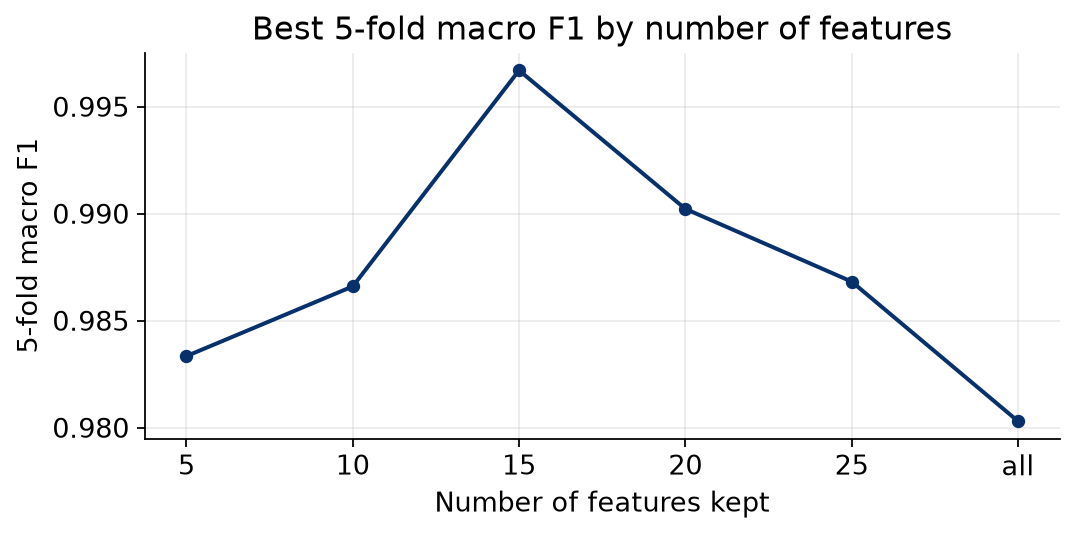
\includegraphics[width=0.44\textwidth]{figures/knn_features.png}
\caption{kNN, 5-fold macro F1 on the training set: all settings with 30 features (left), best score by feature count (right).}
\label{fig:knn}
\end{figure}

\begin{figure}[H]
\centering
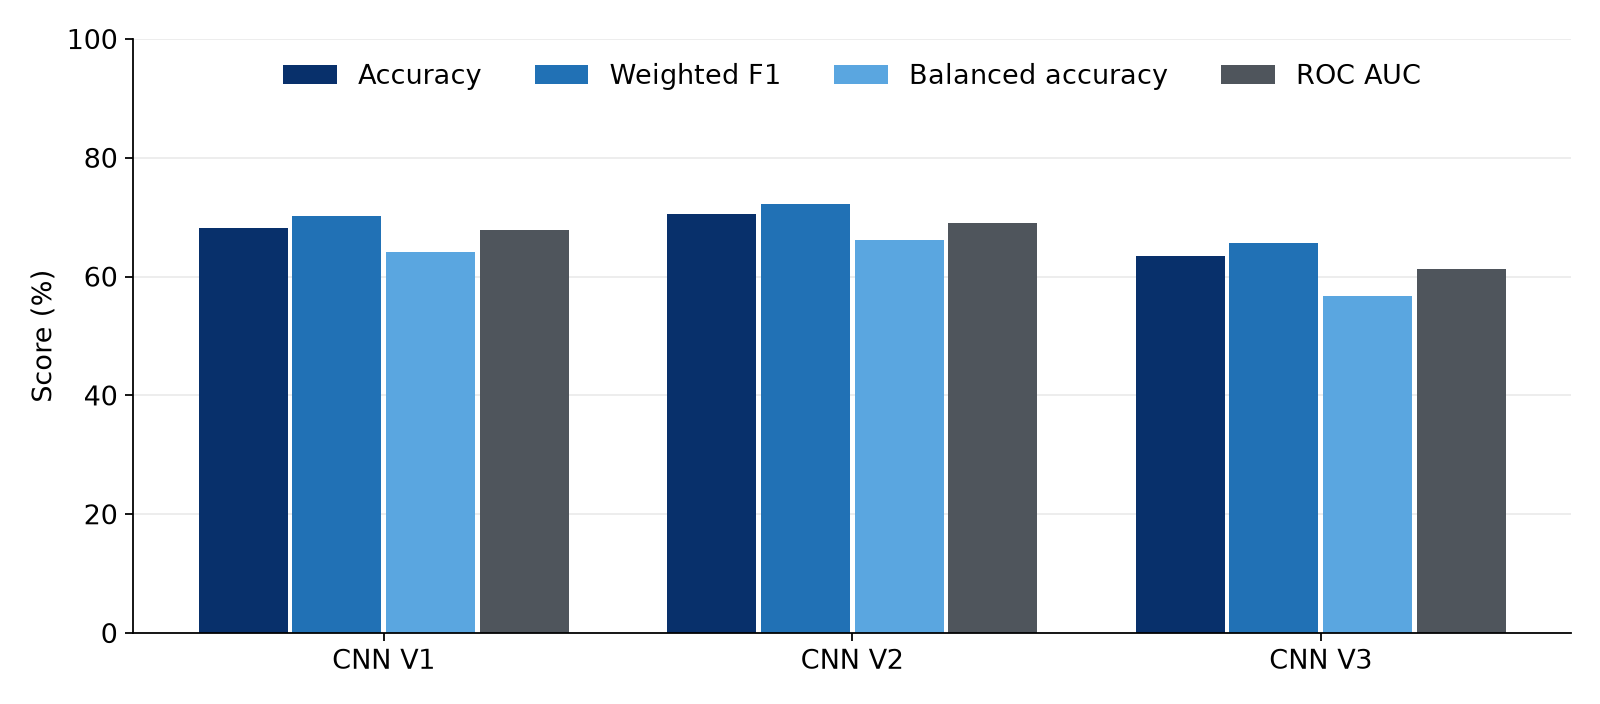
\includegraphics[width=0.75\textwidth]{figures/cnn_comparison.png}
\caption{Validation accuracy, weighted F1, balanced accuracy and ROC AUC of CNN V1--V3 on DS2.}
\label{fig:cnn}
\end{figure}

\clearpage
\phantomsection
\section*{Glossary}
\addcontentsline{toc}{section}{Glossary}
{\footnotesize\setstretch{1.0}
\begin{description}[style=sameline, leftmargin=3.6cm, labelwidth=3.4cm, labelsep=0.2cm, itemsep=1pt, parsep=0pt, topsep=2pt, font=\normalfont\bfseries]
    \glossentry{albumin}{Albumin} A protein healthy kidneys keep in the blood; in urine it is a sign of kidney damage.
    \glossentry{anovaftest}{ANOVA F-test} A score for how differently a feature is distributed in the two classes; used here to rank features.
    \glossentry{ari}{ARI} Adjusted Rand index. Agreement between two groupings of the same patients, corrected for chance (1 = identical, 0 = random).
    \glossentry{bmodeultrasound}{B-mode ultrasound} The standard greyscale ultrasound image.
    \glossentry{balancedaccuracy}{Balanced accuracy} The average of the recall of each class.
    \glossentry{batchnormalisation}{Batch normalisation} Rescaling the outputs of a network layer during training to make training more stable.
    \glossentry{cart}{CART} The standard algorithm for growing a decision tree with yes/no splits.
    \glossentry{ckd}{CKD} A long-term condition in which the kidneys gradually lose their ability to filter the blood.
    \glossentry{cnn}{CNN} Convolutional neural network. A neural network for images that learns small filters applied across the whole image.
    \glossentry{costcomplexitypruning}{Cost-complexity pruning} Cutting back branches of a decision tree that add little accuracy for their size.
    \glossentry{creatinine}{Creatinine} A waste product the kidneys filter out of the blood; high levels mean poor filtering.
    \glossentry{crossvalidation}{Cross-validation} Splitting the training data into parts and testing on each part in turn, with the model trained on the rest.
    \glossentry{cyst}{Cyst} A fluid-filled sac that forms in the kidney and is usually harmless.
    \glossentry{dataaugmentation}{Data augmentation} Training on slightly changed copies of the images, here small rotations.
    \glossentry{dbscan}{DBSCAN} A clustering method that groups points lying in dense regions and marks isolated points as noise.
    \glossentry{decisiontree}{Decision tree} A model that classifies with a sequence of yes/no questions on single features.
    \glossentry{featsel}{Feature selection} Keeping only the features that are most useful for prediction and dropping the rest.
    \glossentry{gaussianmixture}{Gaussian mixture} A clustering model that describes the data as a mix of bell-shaped groups, fitted with the EM (expectation-maximisation) algorithm.
    \glossentry{haemoglobin}{Haemoglobin} The protein in red blood cells that carries oxygen; often low in people with CKD.
    \glossentry{hierarchicalclustering}{Hierarchical clustering} Clustering that starts with every patient alone and repeatedly merges the two closest groups; Ward linkage merges the pair that keeps the groups most compact.
    \glossentry{imputation}{Imputation} Filling in missing values.
    \glossentry{kmeans}{k-means} A clustering method that assigns each point to the nearest of $k$ centres and moves the centres until they settle.
    \glossentry{knn}{kNN} k-nearest neighbours. Classifies a patient by a vote of the $k$ most similar training patients.
    \glossentry{knnimp}{kNN imputation} Filling a missing value with the value taken from the most similar patients in the dataset.
    \glossentry{macrof1}{Macro F1} The average of the two classes' F1 scores, so the smaller class counts equally.
    \glossentry{mutualinformation}{Mutual information} A measure of how much knowing a feature tells us about the class.
    \glossentry{naivebayes}{Naive Bayes} A probabilistic classifier that treats the features as independent within each class.
    \glossentry{outofbag}{Out-of-bag} For each tree of a Random Forest, the training patients left out of its bootstrap sample, which can be used to test it.
    \glossentry{packedcellvolume}{Packed cell volume} The share of the blood made up of red blood cells.
    \glossentry{pca}{PCA} Principal component analysis. Projects the data onto the few directions in which it varies most, here for plotting.
    \glossentry{permutationimportance}{Permutation importance} The drop in a model's score when the values of one feature are shuffled.
    \glossentry{randomforest}{Random Forest} A model that averages many decision trees, each trained on a random sample of patients and features.
    \glossentry{recall}{Recall} The share of the patients of a class that the model finds.
    \glossentry{rocauc}{ROC AUC} Area under the ROC curve. The chance that the model scores a random positive case above a random negative one (0.5 = guessing).
    \glossentry{silhouette}{Silhouette} A score from $-1$ to 1 for how much closer points are to their own cluster than to the next one.
    \glossentry{specificgravity}{Specific gravity} The density of urine; low values mean the kidneys are not concentrating it.
    \glossentry{standardisation}{Standardisation} Rescaling a feature to mean 0 and standard deviation 1.
    \glossentry{stone}{Stone} A hard lump of minerals that builds up inside the kidney.
    \glossentry{stratified}{Stratified} Split so that every part keeps the same class proportions.
    \glossentry{svm}{SVM} Support vector machine. A model that finds the boundary that best separates the two classes.
    \glossentry{transferlearning}{Transfer learning} Starting from a network already trained on another large image set and adjusting it to the new task.
    \glossentry{tumour}{Tumour} An abnormal growth of cells in the kidney, which may be harmless or cancerous.
    \glossentry{urea}{Urea} A waste product of protein breakdown that the kidneys remove from the blood.
    \glossentry{vit}{Vision transformer} An image model that uses attention instead of convolutions to process the image.
    \glossentry{weightedf1}{Weighted F1} The average of the F1 scores of the classes, weighted by class size.
\end{description}
}
